%% (Paper) Campero, 2015- Building cross-language recommendations- a case study.tex
%%
%% Building cross-language recommendations: a case study. 
%% Paper 
%%
%% Gabriel Campero
%% gabrielcampero@acm.org
%%
%%
%% A pdf version of the paper can be easily generated with pdflatex nameofthisfile.tex
%%
%% Here is the series of instructions for generating the file with references:
%%
%% 1: pdflatex \(Paper\)\ Campero,\ 2015-\ Building\ cross-language\ recommendations-\ a\ case\ study.tex
%% 2: bibtex \(Paper\)\ Campero,\ 2015-\ Building\ cross-language\ recommendations-\ a\ case\ study
%% 3: pdflatex \(Paper\)\ Campero,\ 2015-\ Building\ cross-language\ recommendations-\ a\ case\ study.tex
%%
%%
%%
%% This LaTeX file is based on the template:
% This is LLNCS.DEM the demonstration file of
% the LaTeX macro package from Springer-Verlag
% for Lecture Notes in Computer Science,
% version 2.4 for LaTeX2e as of 16. April 2010
%%
%% LaTeX was originally written in the early 1980s by Leslie Lamport (ACM Turing Award, 2013) at SRI International.
%% The current version is LaTeX2e (styled as LATEX2ε). 
%%
%%*************************************************************************

%
\documentclass{llncs}
%
\usepackage{hyperref}
\usepackage{graphicx}
%
\begin{document}
%
\frontmatter          % for the preliminaries
%
\pagestyle{headings}  % switches on printing of running heads
\addtocmark{Building cross-language recommendations: a case study} % additional mark in the TOC
%
\mainmatter              % start of the contributions
%
\title{Building cross-language recommendations: a case study}
%
\titlerunning{Building cross-language recommendations}  % abbreviated title (for running head)
%                                     also used for the TOC unless
%                                     \toctitle is used
%
\author{Gabriel Campero\inst{1}}
%
\authorrunning{Gabriel Campero} % abbreviated author list (for running head)
%
%%%% list of authors for the TOC (use if author list has to be modified)
\tocauthor{Gabriel Campero}
%
\institute{Student, Data and Knowledge Engineering Master's program, University of Magdeburg, OvGU Magdeburg 39106, Germany,\\
\email{gabrielcampero@acm.org},\\ WWW home page:
\texttt{https://github.com/gabrielcc2}}

\maketitle              % typeset the title of the contribution

\begin{abstract}
In this work we consider alternatives for complementing a research paper recommender system, so it can provide cross-language suggestions. To that end we implemented a comprehensive stand-alone prototype targeting German, English and Spanish, and a subset of textual fields (title and abstract). Design choices were based on our review of related work and available tools. We implemented 2 distinct classes of cross-language support based on latent semantic indexing (LSI) and automatic query translation (AQT), respectively. Query expansion (adding synonyms) and user-mediated refinement were incorporated as optional improvements to the latter class. Early tests suggest that our proposal represents a feasible solution to provide the intended functionality and evaluate the different settings. However, at this stage of our research, the prototype still needs to be configured to a more realistic scenario so it can be used for comparing, in a meaningful way, the effectiveness of the different classes of support and optimizing approaches.

\keywords{Cross-Language Information Retrieval, Cross-Language Recommendations, Research Paper Recommender Systems, Cross-Language Latent Semantic Indexing}
\end{abstract}

\section{Introduction}

Together with developments in information retrieval, recommender systems have emerged in recent years as mainstream applications helping users to cope with information overload in several domains, from online shopping to personal email management. Unlike conventional information retrieval tools, where users are expected to put forward specific queries, recommender systems deal with scenarios where users are not required to present an explicit enquiry. Instead, the system produces suggestions by predicting the interest of a user based on past preferences, social context, global relevance of items and other knowledge sources. 

One of the domains where recommender systems have been shown to be beneficial is in aiding academics to carry out literature research. For academics, literature research is not a trivial activity since it involves sifting through a vast number of papers, being produced at such a rate that keeping up with a field can be quite a challenge\footnote{For example Springer Verlag publishes 130,000 articles in their scholarly journals each year (\url{http://www.springer.com/gp/partners/society-zone-issues/shorter-production-times-for-majority-of-springer-journals/4580}).}. Additionally, the papers have to be gathered from diverse digital repositories. Often academics are required to develop criteria for filtering the retrieved documents, so as to deal with the uneven quality of the available material. Furthermore, textual queries might not provide sufficient knowledge, given that the use of alternate terms could obscure the relatedness of topics to a search engine. As a means to complement incomplete findings, academics can also resort to browsing, in a time-consuming fashion, through publication catalogs of specific authors, conferences and institutions. And all of this gets further complicated when being done in several languages that the academic commands. 

These issues make of literature research a highly demanding and critical activity. Any shortcoming can have a damaging impact on the quality of the resulting work. Failures to make good use of knowledge dissemination might lead to insufficiently informed reasoning, missed opportunities, waste of resources in carrying out redundant experiments, among other risks.

Research paper recommender systems (RPRS) are specific software tools proposed to help academics with literature research. Their defining task is to suggest scientific papers to users, aiming to assist them in finding the most relevant and authoritative documents available, overcoming information overload. Citeseer\cite{Bollacker:2000:DRS:630311.630533}, Docear\cite{Beel:2013:IDR:2467696.2467786} and TechLens+\cite{Torres:2004:EDL:996350.996402} are examples of RPRS. 

Additional services (i.e. plagiarism detection, academic alerting services, academic event recommendations, etc.) could be included with a RPRS. However they are tangential to the defining task of RPRS, and thus, will not be addressed in this paper.

One widely unaddressed challenge for existing RPRS is to enable multi-lingual users to simultaneously consider recommendations from digital sources available in all languages they know. To do this, the RPRS has to provide \textit{cross-language recommendations} (CLR). We could define these as suggestions to users where: \textit{a)} the digital repository is mono-lingual, but the fields used to build the recommendations can be in a different language, or \textit{b)} documents in several languages can be recommended simultaneously, while the fields used might be in one or more languages. 

Tools offering this technology could be advantageous to users and service providers, since they represent a medium for improving knowledge dissemination beyond language constrains that might seem arbitrary to polyglot users. However, the real-world gains of this technology are yet to be discovered, since currently there are no mainstream RPRS providing this functionality, and more generally, systems that generate cross-language recommendations are still rare within the recommender systems community.

On the other hand, significant research covering cross-language functionality has been produced by the information retrieval community. Mainstream search engines nowadays offer the possibility of retrieving documents in languages different from the one used in the query. This is known as \textit{cross-language information retrieval} (CLIR) \footnote{Research associations such as TREC's cross-language track (\url{http://trec.nist.gov/}), CLEF (\url{http://www.clef-initiative.eu/}), NTCIR(\url{http://research.nii.ac.jp/ntcir/index-en.html}), FIRE (\url{http://www.isical.ac.in/~clia/}) and the TIDES program (\url{https://ciir.cs.umass.edu/research/tides.html}) have been fundamental in the evolution of cross-language information retrieval technology.}. To support this service, either the query or the documents can be translated. For both CLIR and CLR, instead of using a strict word-for-word translation, a more generic rendering can be employed, based on a bag-of-words containing potential translations. Each of these words can be assigned an associated weight, which serves to signal the most likely translation to the document retriever or the indexer. The weights can be tuned with a knowledge or corpus-based approach.

A common problem for providing CLIR is the lack of knowledge, when based solely on the query string, to perform translation disambiguation. In contrast, CLR could potentially resolve this question by resorting to more extended textual fields. For example, in the case of RPRS, when the title of a paper is not enough for disambiguating a translation, perhaps the abstract might be exploited.

But as there are opportunities in CLR, there are also significant challenges to be addressed. For instance, regarding the architecture of this functionality within the recommender system: will a stand-alone CLIR tool providing input to a recommender system be enough for generating valuable suggestions, or will it be more favorable to embed cross-language features into the knowledge-representation of the recommender system itself? 

Our current research aims to tackle these questions, by studying possible approaches for producing CLR, building upon current knowledge from CLIR. In order to do so, we introduce a CLR implementation for a RPRS, consisting of a stand-alone CLIR prototype, paired with a trivial content-based recommendation scheme. We focus our case study on the German, English and Spanish languages, and a selection of textual fields (namely title and abstract). By this we evaluate some design and implementation choices for the CLR functionality. More specifically we compare two classes of cross-language support. The first is based on latent semantic indexing. It uses cross-language training data to build an index that can be used for querying. The second class is based on query translation, with further improvements.

The remainder of the paper is organized as follows: We start with a brief survey of RPRS, focusing on the textual fields and features commonly used in the production of recommendations, also we try to identify the approaches which might benefit from cross-language support. Secondly, we review selected topics on CLIR, as they pertain to our study. Next we describe our prototypical implementation and some small lab tests performed. Subsequently we assess our early observations, present some related work on CLRS, and to conclude the paper, we discuss some key aspects that might be worthwhile to study further.

\section{Research paper recommender systems}

In their most basic form, research paper recommender systems offer a ranked list of recommendations to each user. This list embodies what the system considers to be the most interesting papers within a repository, for a given user. To produce this list, the system must predict the interest of the user over items from the whole repository. Diverse ideas have been proposed for generating these predictions. We will discuss three main approaches that are amiable to be enriched by cross-language support. 

\textit{Content-based filtering} (CBF) is one of the most predominantly used in RPRS\cite{beel2014research}. It assumes that users are interested in items similar to their previous interests.  Consequently, a model of the user can be formed by considering a collection of documents from those previous interests. This collection can be discerned by the system based on recorded transactions: documents the user browsed, downloaded, authored, rated, etc. Fields from documents in this collection (title, abstract, meta-data\cite{nascimento2011source}, and so forth.) are then used to build a set of features which can be further weighted according to their discriminative powers, domain/lexical concepts and/or user feedback \cite{lops2011content}. Finally they are combined to form a resulting user model, which aims to represent the user's interests in a content-based space. Given that all documents can also be mapped to this content-based space, the user model can be compared for similarity with the entire document repository, so the list of most similar documents can be produced.

On a user-as-author approach, the papers by the user can be also analyzed for citations, which are then included into the user profile, so as to better characterize the user \cite{sugiyama2010scholarly}\cite{strohman2007recommending}. 

Apart from the classical TF-IDF vector-space measure, similarity can be represented as a constrained measure or using citation-based relatedness, among others\cite{bollacker2000discovering}. 

One positive characteristic of the CBF approach is that it can give feedback to users explaining the causes for the recommendations, which can in turn increase user satisfaction with the system.

Nonetheless, there are several critiques to the CBF approach. Perhaps the most important is the problem of limited content analysis: feature representations can only capture a limited part of the user's perception of the text, dismissing valuable aspects such as the popularity of the publication, the quality of the research, it's authoritativeness, novelty, etc. Another critique is that classical CBF implementations can over-specialize the recommendations w.r.t. past preferences, and not allow for serendipitous discoveries. Some solutions to this issue have been proposed for general RS, introducing randomness\cite{sheth1993evolving}, filtering out items that are too similar to be relevant\cite{zhang2002novelty} and using domain/lexical concepts \cite{sugiyama2014comprehensive}\cite{iaquinta2008introducing}.
CBF has also been criticized for it's use of implicit feedback, which can misrepresent the user's interests\cite{balabanovic1997fab}.

A second approach to RPRS is \textit{collaborative filtering} (CF). The fundamental idea behind it is that users might be interested in items that "similar" users have found to be interesting. Predicting similarity is thus the first task for this approach. It can be accomplished through several means, such as considering explicit ratings from each user. These are then employed to construct a user-item matrix, where each entry quantifies the relation between a user and an item. Methods such as k-nearest neighbors can be applied to this matrix, to determine the closest neighbors of any user, and then the final recommendations can be formed by taking into account items unknown to the user, and multiplying by the number of votes they have received from the neighbors. Other possible methods for finding the neighbors include clustering and bayesian networks.

Unlike CBF, CF provides a chance for serendipitous discoveries, since recommendations come from other users, emulating traditional word-of-mouth recommendations. The human factor can also contribute to the quality of the recommendations.

A problem of the CF approach is that when relying exclusively on explicit ratings, the resulting matrix can suffer from data sparsity, given that users commonly lack incentives for giving explicit ratings. Sparsity is also something intrinsic to the RPRS domain, which perhaps decreases the appropriateness of this approach for the domain. For some research paper recommender systems sparsity has been found to be of three orders of magnitude higher than that of traditional movie RS\cite{vellino2013usage}. 

The most extreme case of sparsity occurs for new users: there is nothing rated yet, so no recommendations can be made. This situation is known as the cold-start problem. To alleviate this, other information can be considered by the recommender system. Implicit ratings could be devised based on diverse interactions of the users with the documents\cite{pennock2000collaborative}\cite{yang2009cares}. However this decision can undermine the human factor of user recommendations, since the implicit ratings can fail to represent user intentions.

Implicit ratings that are somehow more reliable can be discerned by the use of citations: following an user-as-author approach, the papers cited by the user can be added as positive ratings to the matrix, so users that cite or have rated similar papers can be chosen for producing the recommendations\cite{caragea2013can}\cite{mcnee2002recommending}. 

In general the use of citations as a knowledge source for building the recommendations is a key element of the domain of research papers, since unlike other domains where the items can be unrelated, there exists a meaningful web of citations that links an item to others as soon as it enters the system. Highly specialized methods exist for analysis of the citations and their context, such as latent-topic models\cite{blei2003latent} and the pair-link-LDA and link-PLSA-LDA model\cite{blei2003latent}\cite{he2009detecting} (which aim to predict relationships between citations). Another family of models are the translation-based citation recommendation models (matching the descriptive language of the citation context with the more structured language used for including the citation in the bibliography)\cite{huang2012recommending}\cite{lu2011recommending}. 

Unfortunately the use of citations can be an error-prone task when this information is not supplied as meta-data to the document. On this case, content extraction is more difficult than for regular text, since the bibliography and the references have to be automatically and univocally identified, discerning their specific sub-fields\cite{councill2008parscit}. A mistake in this extraction has a high probability of producing a misrepresentation of the document. 

A less obvious approach for RPRS, based on CF, is to produce an item-item ratings matrix. Each document is modeled as if it were a user, and their transactions with other items (being read together in a same session\cite{bollen2006architecture}\cite{hwang2003prototype}\cite{monnich2008adding}, cited together\cite{mcnee2002recommending}, downloaded together\cite{pohl2007recommending}, etc.) are seen as ratings. Consequently, documents that have a similar set of ratings under this representation can recommend documents to one another. In order to connect this approach to the users, all documents from a user have to be mapped to that item-item representation, so as to get partial recommendations, which are then merged, and the most voted can be returned. This approach can be considered to be a special form of CF, but it can also be treated as another approach, called \textit{co-occurrence analysis COA} or item-centrism. 

The key idea behind COA is that two papers are the more related the more they are cited together. By representing relatedness instead of similarity, the results from this approach can be more serendipitous than CBF. However the use for this approach is not always possible, since for some repositories co-citation between in-repository items might not be commonly found.

Apart from these three approaches we can also mention\textit{hybrid RPRS}. They represent a fairly common approach, built on combining features from different approaches \cite{sugiyama2014comprehensive}\cite{dong2009digging}. TechLens is a primordial example of a hybrid RPRS combining ideas from CF and CBF\cite{ekstrand2010automatically}.

In general, under all the approaches described, the fields that are analyzed for building the features can be textual or non-textual. They can also be intrinsic to the document files (requiring extraction) or external to them (as meta-data or as global variables provided by the repository). Textual fields are commonly represented at word or syntactic levels, such as the title of the document, header, abstract, introduction, foreword, author-provided keywords, the body of the document, annotations, citation and citation context. Lower morphological representations of the features can also used, such as n-gram models\cite{ferrara2011keyphrase}. Some fields could also be assigned to the document from a semantic level. This refers to knowledge about entities such as authors, topics \cite{jiang2012recommending}\cite{bethard2010should}, position in a scientific classification tree or mind-maps where the users have meaningfully described some of their ideas about the documents. 

Non-textual data, such as writing style and layout information has also been used to enrich the document representation.

From our short review on the different approaches for RPRS we can infer that the CBF approach is the family of methods most likely to be benefited from cross-language support, with word and phrase level fields being the most likely translation candidates. Knowledge fields are also possible candidates, and for this case, special care should be taken so the translation allows to losslessly map information between the knowledge webs that the recommender might have for the different languages.

One significant problem we observed refers to the use of fields extracted from within the document file. Given that for RPRS the files have to be processed and converted to text, important fields can be mis-captured, leading to faulty behavior. A mistake at this stage could be amplified if the text is further translated, and it's impact could be wider according to the field in which it appears (i.e. a mistaken translation of a word in an abstract would perhaps have less effect at matching time than a mistake in the title). The use of hand-checked meta-data as an input could be more beneficial for CLRS, since it would mean that the process can start with more reliable data. This however was not tested in the current project.

On the following section we will further elaborate on these observations, as we introduce cross-language information retrieval.

\section{Cross-language information retrieval}

The domain of CLIR is perhaps too wide to be aptly described in a short section\cite{nie2010cross}. For this reason we will restrict to presenting in a general manner two approaches used in this domain: Latent Semantic Indexing (LSI), which is perhaps the most simple to understand method from a family of approaches to the CLIR task, that are called topic models. This family is characterized by their aim to distinguish underlying topics from documents in a given term-space. 

Next, we will shortly discuss automatic query translation (AQT), trying to focus on the most fundamental aspects. We can define AQT as a very broad approach to CLIR that can be ultimately characterized by it's being based on a similar combination of services and optimizations at different levels, such as described (following ideas from Ahmed and N\"{u}rnberger, 2008\cite{ahmed2008arabic}) in Fig. \ref{fig:AQTWorkflow}. 

\begin{figure}[h!]
  \centering
      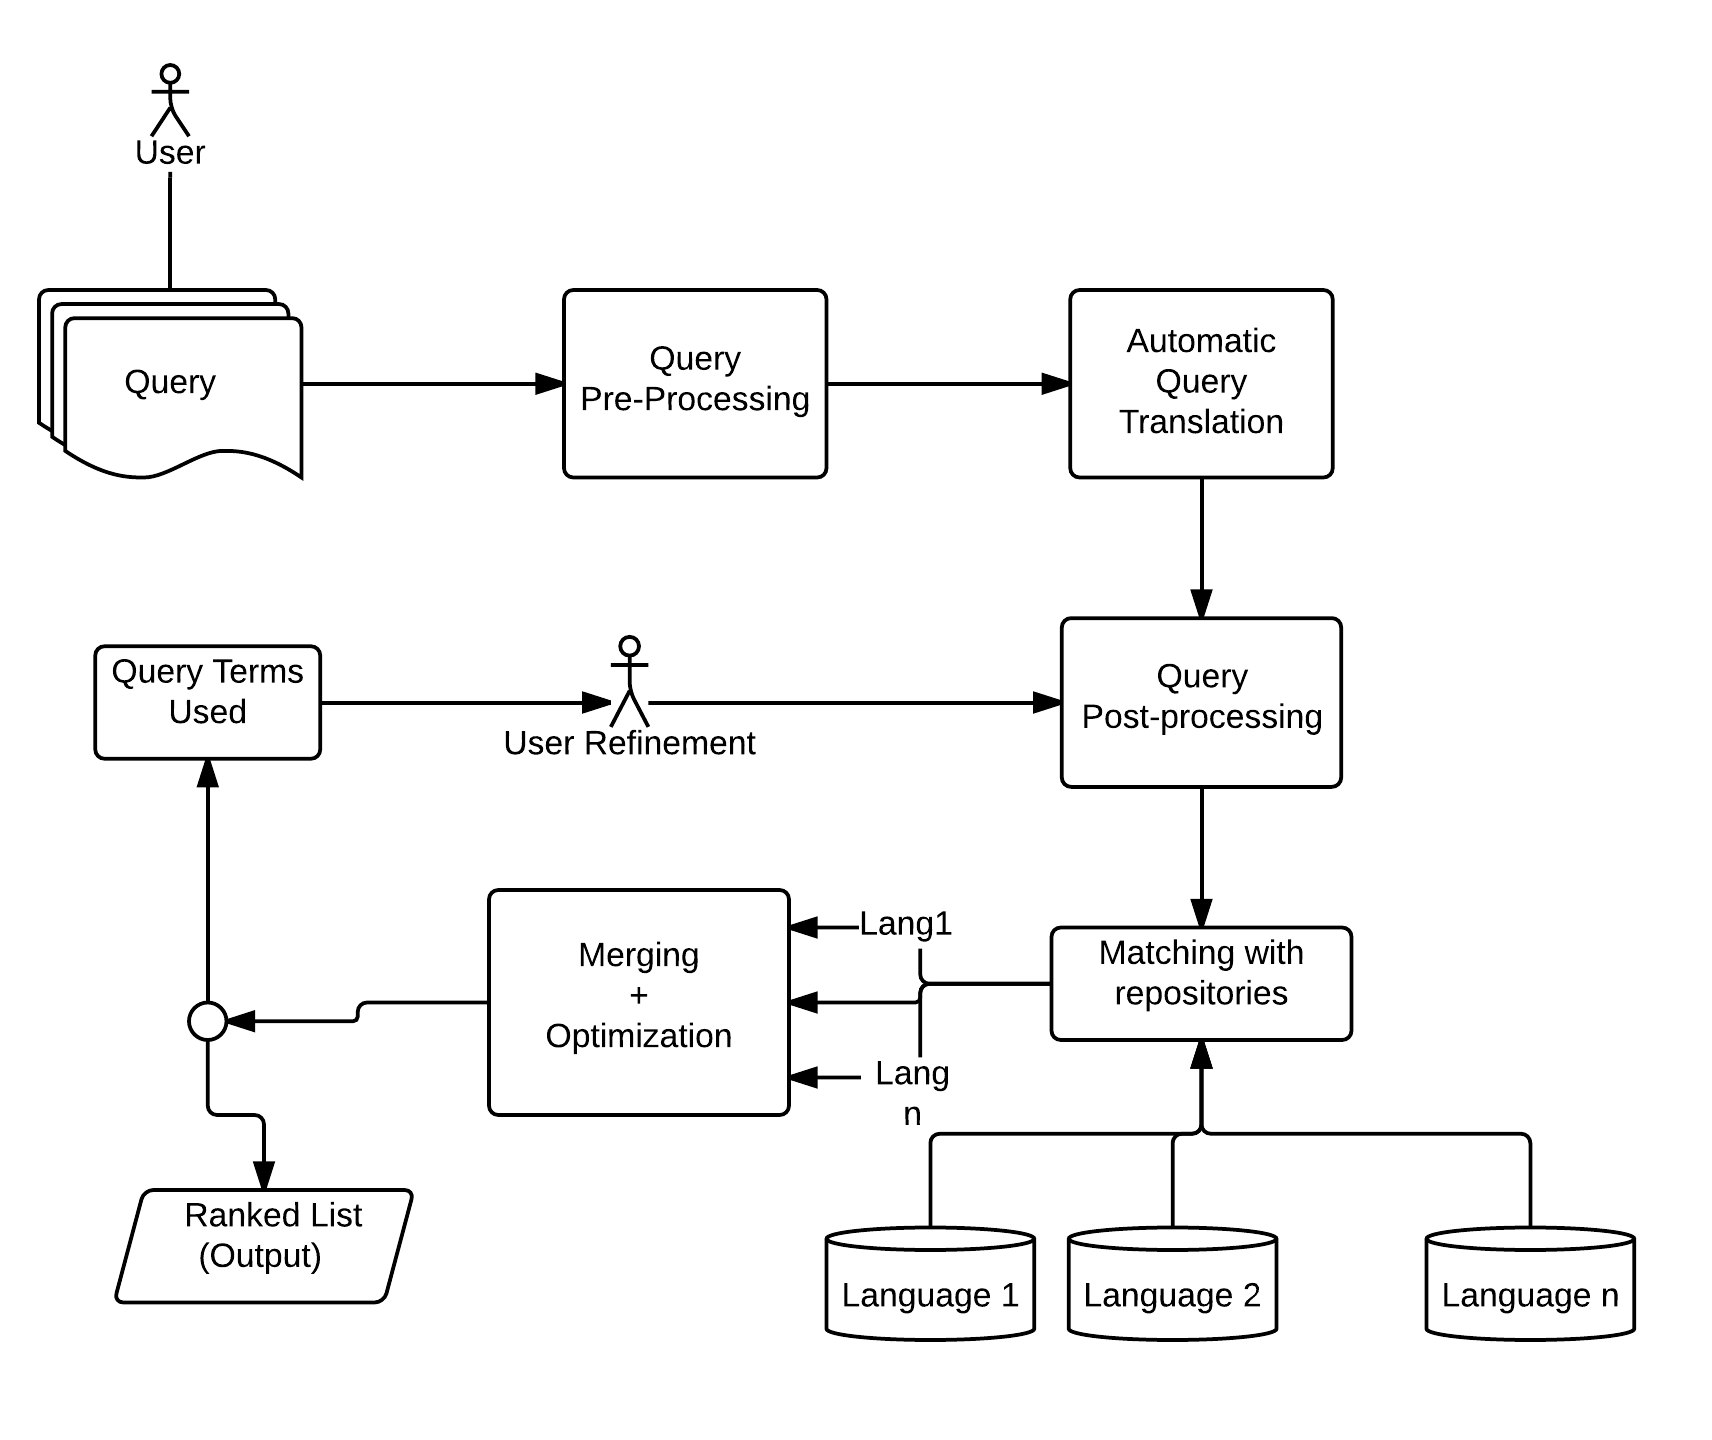
\includegraphics[width=0.7\textwidth]{AQT.png}
  \caption{Automatic query translation workflow.}
\label{fig:AQTWorkflow}
\end{figure}

\subsection{Cross-language latent semantic indexing}

Latent semantic analysis, also called Latent semantic indexing (LSI), is a theory for extracting meaningful relations between sets of terms. This meaning is estimated by statistical methods using a large corpus of text\cite{landauer1997solution}. LSI has been extended to cross language applications, conforming an approach called CL-LSI\cite{dumais1997automatic}. On this approach the processing initially defines a semantic vector space based on cross lingual training data. From a corpus of concatenated parallel multilingual documents, various terms and their frequencies are computed to form a term-frequency matrix. This matrix is then decomposed using matrix factorization to get three matrices, which are described in Fig. \ref{fig:LSI}.

\begin{figure}[h!]
  \centering
      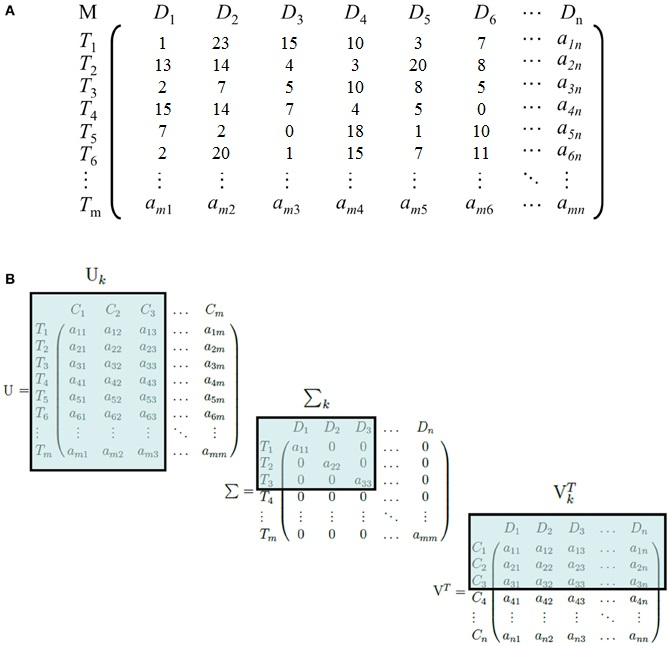
\includegraphics[width=0.7\textwidth]{LatentSemanticIndexing.jpg}
  \caption{Matrix factorization for multi-lingual training data with LSI.}
\label{fig:LSI}
\end{figure}

The U matrix represents the relation between the multi-lingual terms and the semantic dimensions. The Sigma matrix (at the center) is the kernel of the decomposition, while the Vt matrix represents the relation between documents and the semantic dimensions. If we perform a ranked reduction to k entries, along the main diagonal of S, we should obtain a representation of the k most important orthogonal meanings (shaded blue in the figure).

After these semantic space has been established we can perform the indexing, which is stored in a different matrix. Under a controlled vocabulary approach, no new terms would be added during indexing. So, as shown in Fig. \ref{fig:IndexingLSI}, the new documents that need to be indexed are first represented according to their frequency of terms from the controlled vocabulary. This matrix is then mapped to the semantic dimensions by multiplying by Uk and the inverse of the Sigma matrix from the previous step. This process is called "folding-in". Subsequently, all the documents are combined to form a matrix where each column is a vector representation of the document in the semantic space, obtained from the training data. 

\begin{figure}[h!]
  \centering
      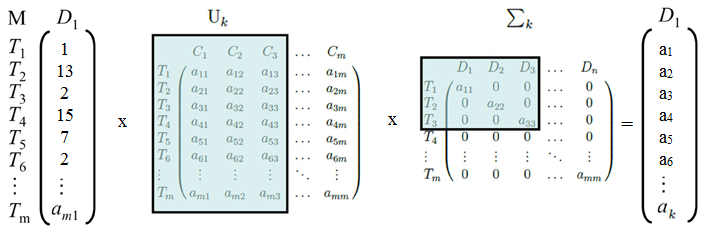
\includegraphics[width=0.7\textwidth]{LSI.png}
  \caption{Indexing with LSI.}
\label{fig:IndexingLSI}
\end{figure}

The queries from the user can also be mapped to the semantic space using the same methods as seen in Fig. \ref{fig:IndexingLSI}, so as to compare them against the documents using a similarity or distance measure such as cosine similarity. In this way cross-language queries can be supported without explicitly translating the query terms or the documents.

This approach has been studied for several standard collections and found to perform fairly well for finding documents in one language by querying in another language, while overcoming the polysemy problem (difficulty of distinguishing several meanings of a word, which under LSI are better defined through the mapping of the word and its context to the semantic dimension)\cite{dumais1997automatic}. 

Further approaches exist so as to map multi-lingual terms into language-independent latent semantic domains. These approaches are generally called topic models approaches. Latent Dirichlet allocation (which was already mentioned, as it has also uses in specialized citation analysis, as in the Link-PLSA-LDA)\cite{vulic2013cross}, LSA with non-negative matrix factorization, oriented principal component analyis, coupled probabilistic LSA\cite{platt2010translingual} are some of them\cite{arora2012learning}. 

A significant issue for the use of LSI is the need for a suitable parallel corpus, and the dependence of the results on this factor. Since comparable corpora (for example Wikipedia pages for a same topic in different languages) are more common than parallel corpora, several studies have been devoted to adapting topic model approaches to the use of these corpora\cite{vulic2013cross}.

\subsection{Automatic query translation}

For CLIR, several settings exist regarding what should be translated (the documents, the queries, both to a pivot language, or none). Query translation is the most common of the settings, since document translation is a much more process-intensive task. It is also a more generalizable approach than some methods that don't use translations, but instead, for example, treat French as a bad spelling of English, during the searching.

On general terms, while machine translation (which is used for document translation) might require a precise word-for-word translation, where each term has to be disambiguated so as to be adequately transferred, while at the same time aiming to preserve the synctactic structure. Query translation would not require such a strict language transfer. Instead, it could aim at the most probable meaning, and still be able to produce good retrieval results. This is the motivating idea behind a series of approaches to the query translation task, which are based on a weighting of a bag-of-words of possible translation alternatives\cite{ballesteros1998resolving}. In this way, CLIR can be based on a more imprecise translation of the queries, done by machine-readable dictionaries, knowledge-based methods (using semantic nets with interlingual representations, such as EuroWordNet or Multi-WordNet) or based on statistical methods, using parallel or comparable aligned corpora. 

Some key challenges in all configurations of query translation are out-of-vocabulary words (produced by insufficient lexical coverage) and translation ambiguity. These issues could be addressed with semantic means, during pre and post translation stages. 

Other problems that query translation needs to address are language specific characteristics which might damage the results. Often decompounding, conflation of words with the same root, correction of spelling errors could be applied at a pre-processing stage, to improve the results of the resulting translations, and thus of the retireval\cite{ahmed2008arabic}. Even spelling correction, and user-mediated indications of the correct sense of provided queries or entity recognition can have a positive impact on the results\cite{de2004ontology}. 

Given this description of the phases needed for query tranlation, the AQT approach can be finally described as a combination of stages and potential optimizations at each one of them, as seen in Fig. \ref{fig:AQTWorkflow}.
We will not discuss further about the potential approaches to AQT improvement thorugh it's phases, but some possible methods are presented when we discuss the prototype.

Before concluding this section we have to mention that combinations of AQT and latent approaches have also been proposed, and found to be more beneficial over standard TREC-tests than any stand-alone version\cite{roth2010combining}. 

\section{Prototypical implementation}

\begin{figure}[h!]
  \centering
      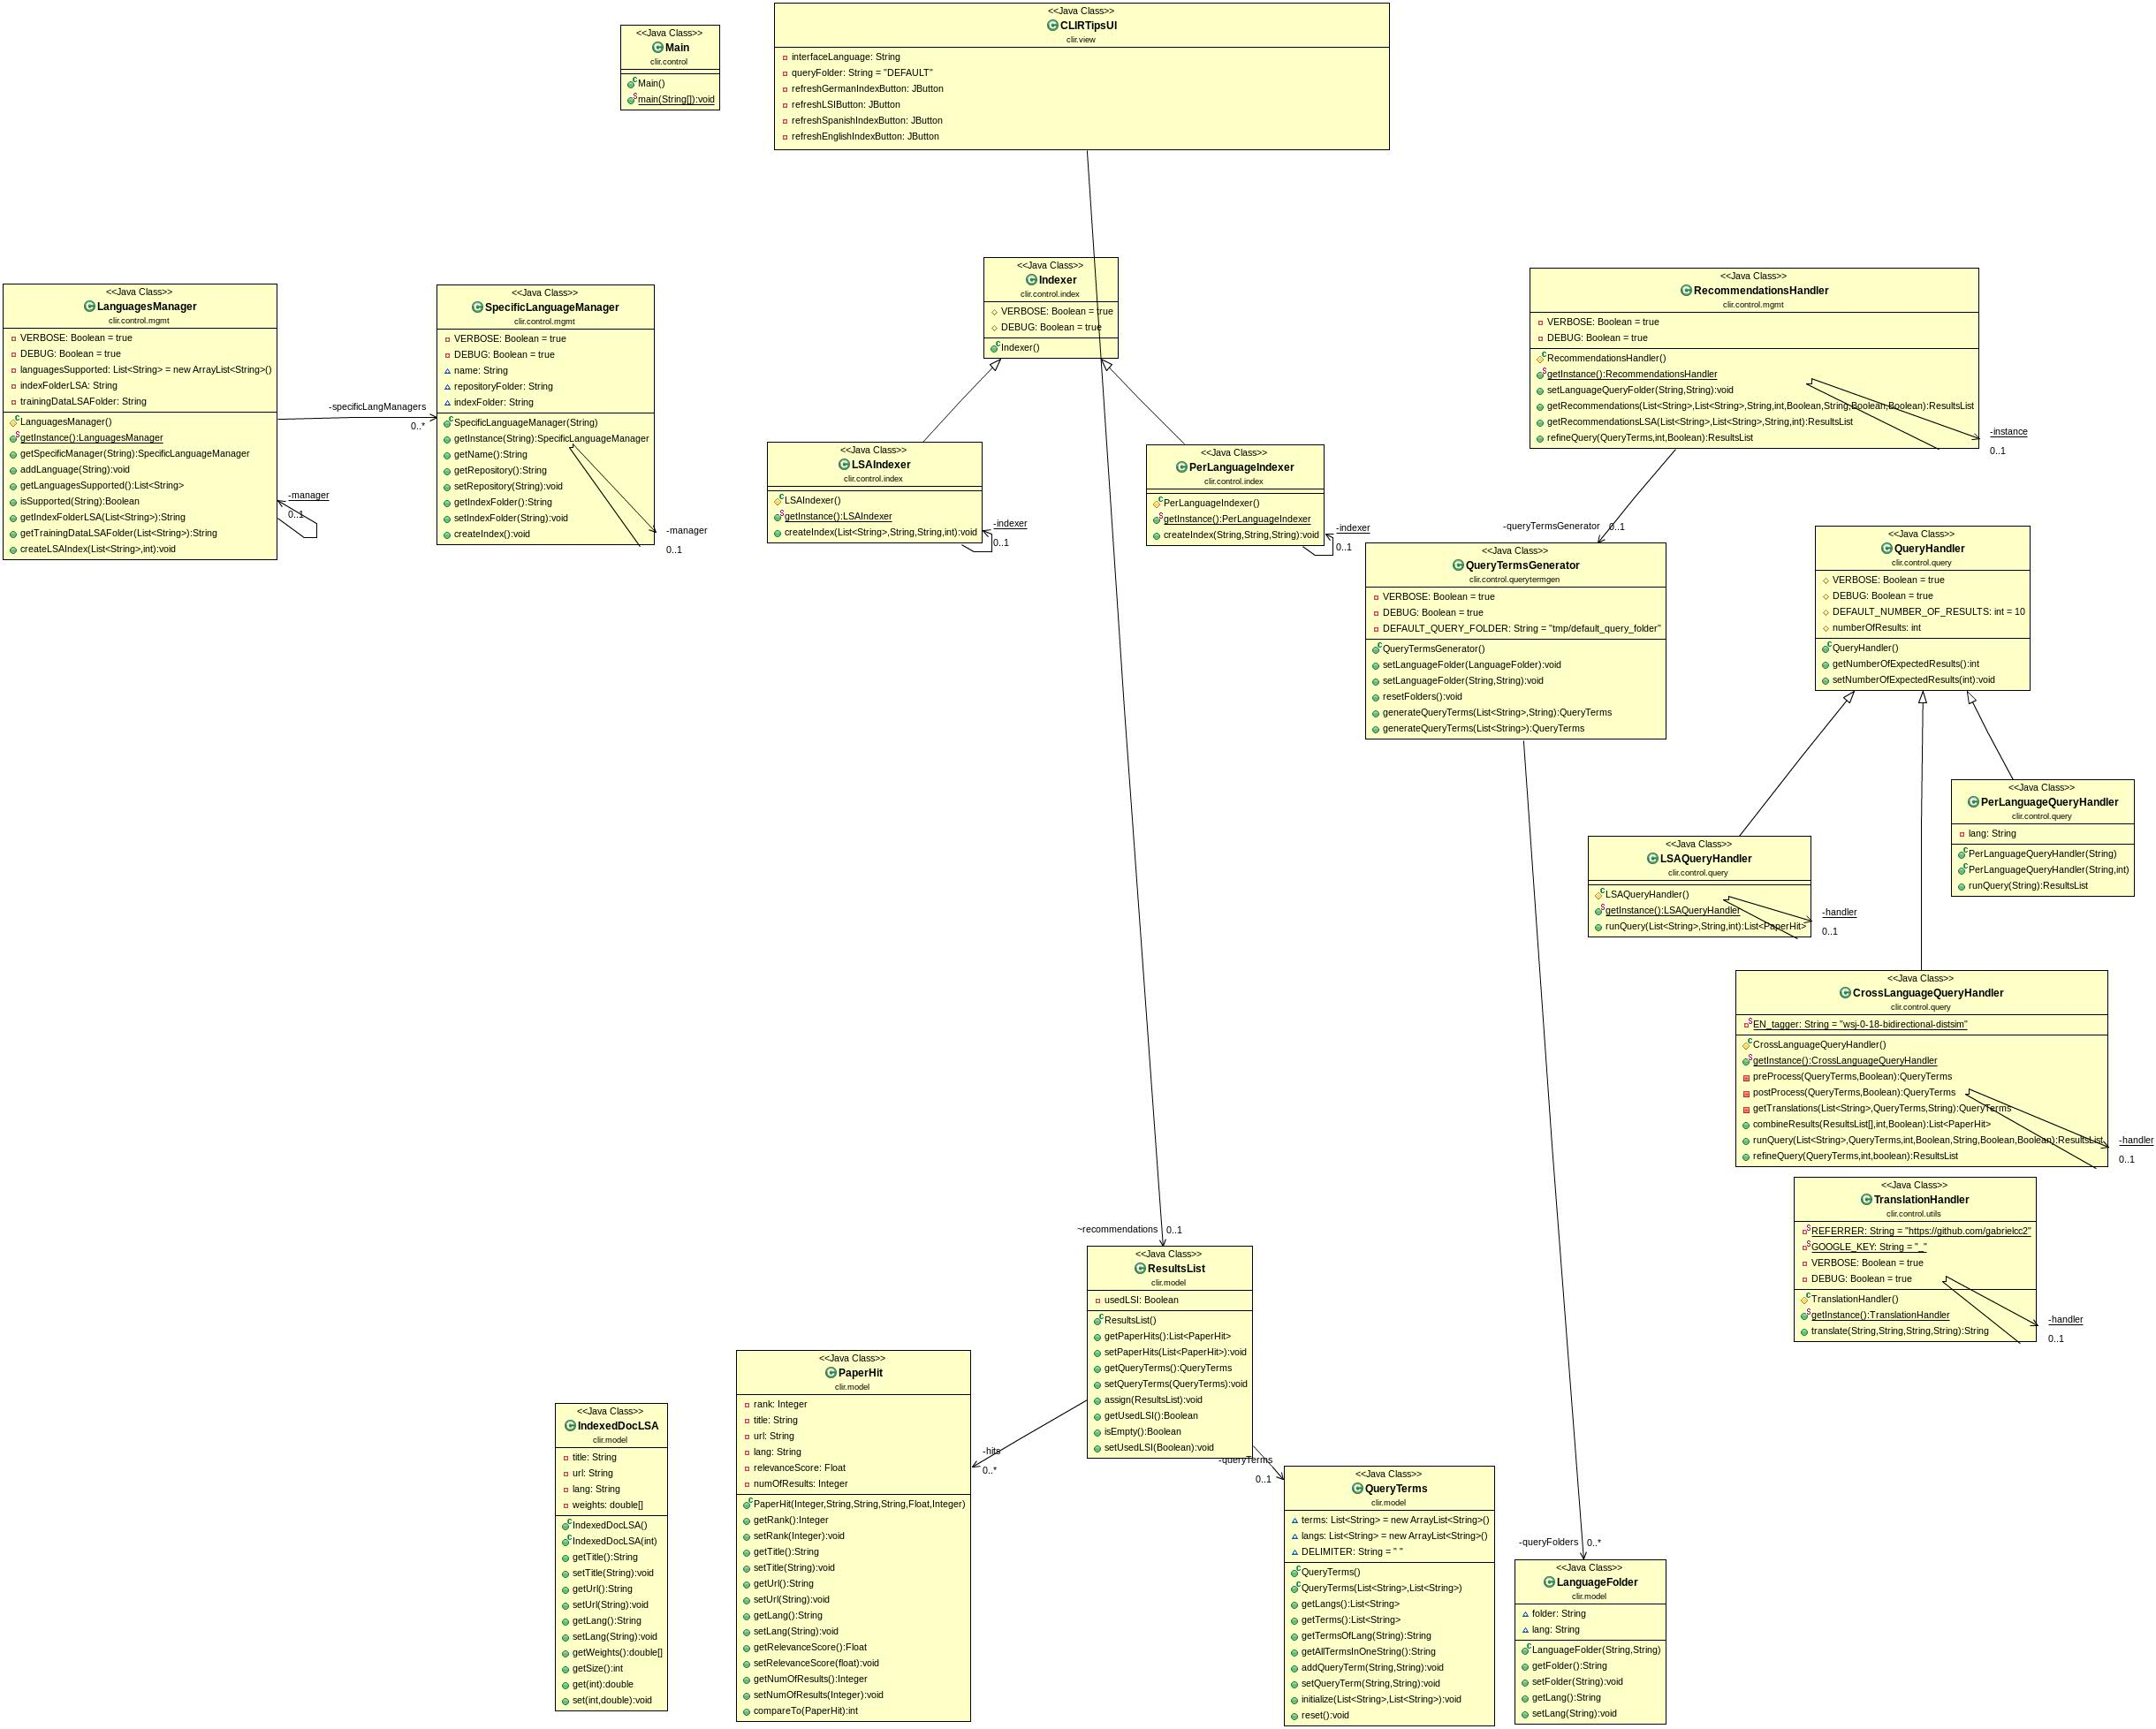
\includegraphics[width=0.9\textwidth]{CLIRTipsUML.jpg}
  \caption{Architecure of CLIR Tips}
\label{fig:ClirTips}
\end{figure}

As a way to evaluate the intended cross language functionality, we developed a prototype written in Java for German, English and Spanish recommendations. It is made available on the Web \url{https://github.com/gabrielcc2}. Our prototype offers the two main approaches to CLIR: Topic model based querying, through latent semantic indexing; and automatic query translation. We chose to include in our prototype automatic query translation since it represents a "standard" workflow for CLIR, allowing to combine alternative optimizations at several processing stages. On the other hand LSI was chosen, because we speculated that perhaps, given an appropriate corpus, it's controlled vocabulary approach might be useful for capturing language-independent characterizations of research study fields, thus providing an easier and less error-prone approach to recommending papers from a given study field. 

Additionally we thought that a study of both techniques through a same tool might be positive so as to allow us to study further ahead alternatives for complementing the techniques, and perhaps using one for some specific recommendation task, and one for others.

The approaches we studied are embedded within a very simple CBF approach that scans user folders so as to generate queries based by representing users as a concatenation of their documents. Title and abstract were used as fields for indexing, but only the title was used for querying, since it was a more reliably extracted field for documents in German and Spanish. This could be improved upon.

The first step that our prototype considers is term extraction from PDF files. This is accomplished by using a tool called PDF-Inspector (\url{https://github.com/Docear/PDF-Inspector}). We chose title and abstract as the two fields most suited for preliminary testing at this stage. To detect the abstract, we relied on an empiric approach, detecting descriptive terms from each language. A simple cleaning scheme removing some non-letter characters was set in place.

LSI was implemented by using the Apache Math commons library (\url{https://commons.apache.org/proper/commons-math/}), under the same controlled vocablulary setting that was described in section 3.1. We developed classes LSA indexer and LSA query handler (see Fig. \ref{fig:ClirTips}) to support this functionality.

Several available sources were considered for LSA cross-lingual training data, but at this stage we decided on a custom implementation as the most suited for a simple study. 

A comprehensive scheme was devised so as to allow AQT. It was based on the workflow described in Fig. \ref{fig:AQTWorkflow}. Singleton classes, LanguagesManager and SpecificLanguageManager were implemented to keep track of the state for each language (location of indexes, repositories, load-state, etc.). 

For the indexing itself, a traditional approach was championed using Lucene. 

Querying was implemented using the same processing workflow described in Fig. \ref{fig:AQTWorkflow}. Most of this is implemented in the CrossLanguageQueryHandler class. The first step is pre-processing. No optimizations were performed at this stage, but separate functions were included in the architecture so as to support future initiatives.

Three translation services were supported: Aperitum Java API (\url{https://github.com/rmtheis/apertium-translator-java-api}) coupled with the Aperitum web service (\url{http://api.apertium.org/}), Google translate API (\url{https://code.google.com/p/google-api-translate-java/}) coupled with Google Translate web service (\url{https://cloud.google.com/translate/docs}); and a Moses statistical translation system (\url{http://www.statmt.org/moses/})\cite{koehn2007moses}, which can be built using parallel and comparable corpora. These have to be aligned using an alignment predictor, which can be implemented using GIZA++ (\url{https://code.google.com/p/giza-pp/}). Further characteristics of this translation service can be configured. 

Note that all of these services are provided to our program in a server-based architecture, with Apertium and Google being web-based, and Moses being socket-based, while running as a process in the background.

Support for connecting to the translations services is embodied in the TranslationHandler class. 

For query post processing we considered query expansion by adding synonyms from synsets drawn from the Multi-WordNet ontology\cite{pianta2002developing}, which we managed to run as a SQL database in a MySQL server. 

To ensure that the correct ontology (Verbs / nouns, etc.) is queried, we use the Stanford System of part of speech tagging (\url{http://nlp.stanford.edu/software/tagger.shtml}), with a specific tagger for each corresponding language. 

Expanding the query with synonyms enables the system to find matches for a broader set of query terms. It also aims to reduce potential errors from sub-optimal translation output. 

The matching is then done in the traditional way using Lucene with a boost of 1.5 for every title hit. Stopword elimination and stemming are left to the Lucene language-specific analyzers. 

An optional optimization was devised at merge-time, allowing to boost documents from given languages, under given conditions. This idea might permit potential extensions in the future. Most particularly it can serve to boost hits in under-represented languages, or according to user language preferences regarding topics.

A multi-lingual GUI was built to enable easy consumption of results, while keeping in mind possible users and a coherent view of how the product could be used. The GUI was considered to be crucial so as to facilitate testing an additional service: user-mediated query refinement, through which the system can be momentarily queried as an academic search engine. This is an option that is provided after getting the first recommendation set. At this point, the user could inspect the query terms that the system produced to generate the recommendations. Then the user could also refine the terms and request new recommendations.

\begin{figure}[h!]
  \centering
      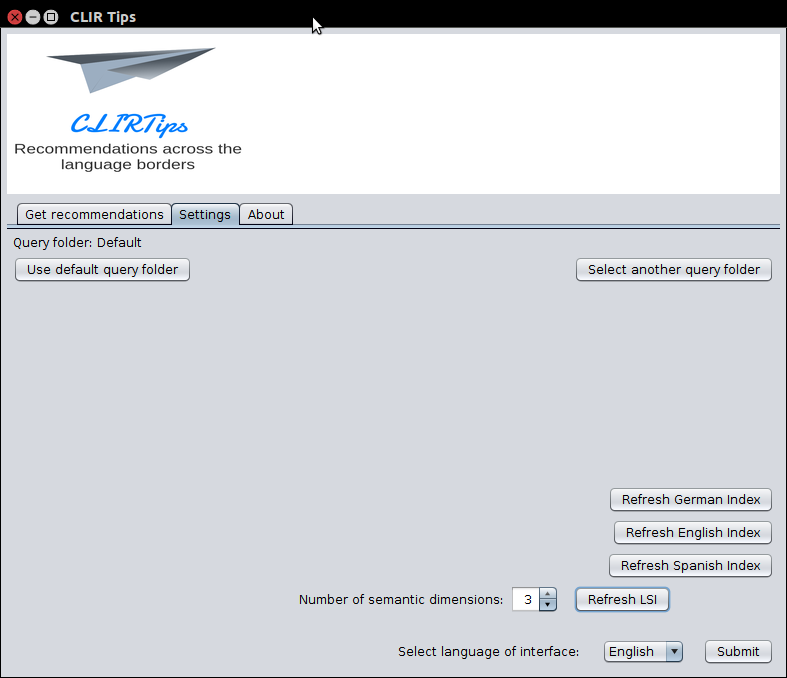
\includegraphics[width=0.5\textwidth]{Settings.png}
  \caption{Settings.}
\end{figure}

\begin{figure}[h!]
  \centering
      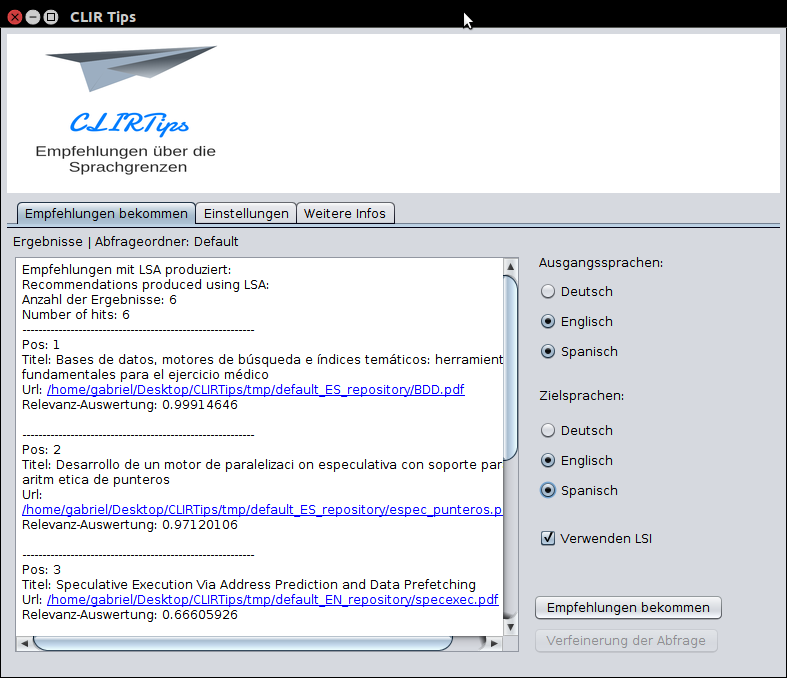
\includegraphics[width=0.5\textwidth]{ResultsLSI.png}
  \caption{Results from LSI.}
\end{figure}

\begin{figure}[h!]
  \centering
      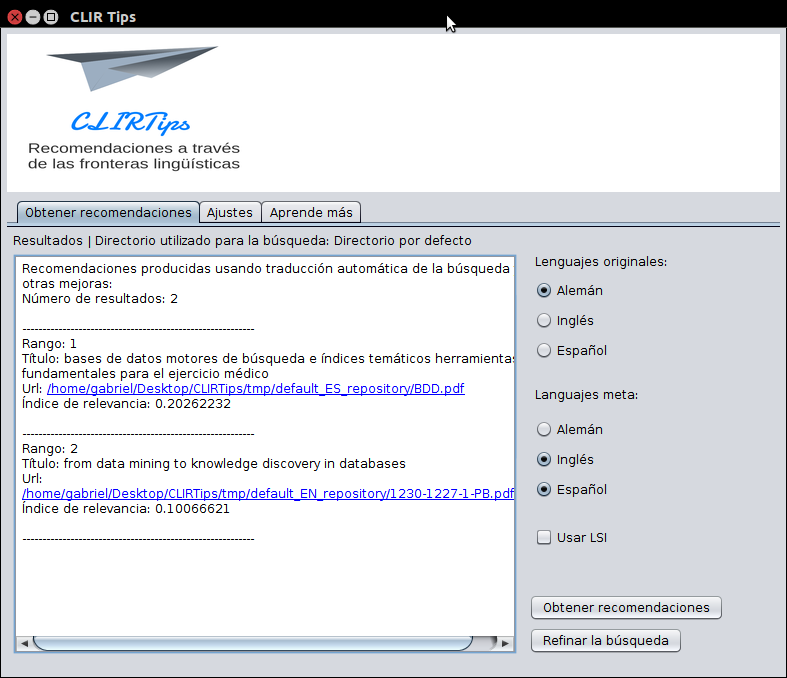
\includegraphics[width=0.5\textwidth]{Results.png}
  \caption{Results from automatic query translation.}
\end{figure}

\begin{figure}[h!]
  \centering
      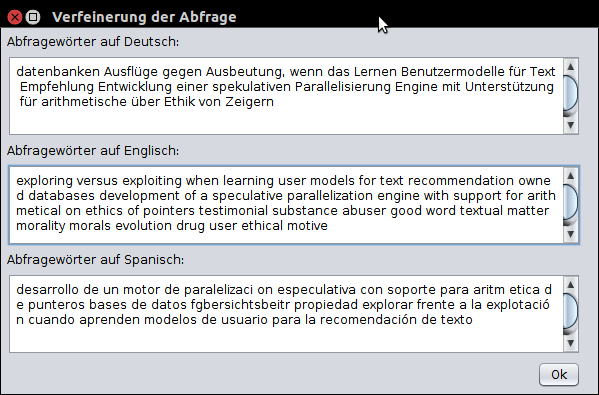
\includegraphics[width=0.5\textwidth]{Refinement.png}
  \caption{Refinement of query terms.}
\end{figure}

\section{Discussion}

At this stage we consider that our system represents a simple framework that could be used as a starting-point for comparing cross-language services happening during different processing phases, and their contribution to the end results. However, at this stage of our research, for this evaluation to be meaningfully and realistically done, special aspects need to be addressed. These issues will be discussed in this section, for they represent the core of our insights at this stage of the research.

The most striking problem was in our use of the PDF-extractor tool: some word omissions and splitting of terms was found when dealing with non-English characters present in German and Spanish terms. Since the results from this tool are the input to the rest of the system, it is fundamental to improve it's use, or to decide on testing while using well-extracted data (such as hand-checked meta-data).

For LSI, the crucial issue is the need for using a standard and representative corpus as training data. This corpus must also be adequate for the topics of the research papers in the RPRS.  Apart from this, some of our design choices, such as not allowing new terms after training, can be revised. Also, given our architectural proposal, LSI could be easily replaced with LDA or other models, which could be studied to compare which provides a better support or adapts better to the corpus in use.

With regards to AQT, we found that it's results seem to depend on much more factors than the results of topic models, and also, by using a stack of services, the results can be more time consuming than the other approach (which instead of relying in services spends most of it's execution time in matrix calculations, that could also be time-consuming), specially for longer queries. However, AQT seems to present some advantages w.r.t. LSI: it might be more scalable w.r.t. the number of terms in the vocabulary, and additionally, by providing explanations and allowing fine grained query refinements, they might increase user satisfaction with the system.

The potential benefits of query expansion as an optimizing technique are not accurately represented in our prototype, since at this point it only uses an English WordNet. Other flaws of our representation is that since we haven't included a Name Entity Recognition service, and we expand on a word-by-word basis, we can fail to capture the synsets of entities that span several words. For example, a "kitchen aid" may be expanded by our prototype as "bakery charity", when "kitchen utensil" might be more appropriate.

Additionally, by not including a Word Sense Disambiguation service, and instead querying for the most common of senses, we are perhaps introducing noise into our results, and still not expressing the potential improvements which could be reached by using the extended context which is available to RPRS, and not necessarily available to traditional IR systems.

Once the aforementioned issues have been solved, proper testing could be carried out with our prototpe, using appropriate standard benchmarks, so as to generate insights on how well the approaches perform for generating recommendations, and how they could be adapted to existing and more complex recommending schemes.

\section{Related work}

A limited number of published proposals exist for CLRS, and an even more limited number exist for CLRPS. On this section we will consider the proposals we have found, so as to better characterize the state-of-the-art regarding the use of cross-language functionality within recommender systems.

Generally speaking, we found some published proposals based on inter-lingual semantic knowledge, others based on topic-models and others are able to exploit cross-language elements from repositories, without the need for translation.

Mars\cite{lops2010mars}, is a proposal based on inter-lingual semantic knowledge. It is a multi-language recommender system for movies. By using Multi-WordNet next to a Word-Sense Disambiguator, the authors are able to map the description of each item, first into the ontology representation of the language of the description, and then to the inter-lingual, or language-independent expression of the term. In the end, all items are mapped to this language independent domain, so as to allow cross-language functionality. This approach can be considered to be more similar to dictionary-based translation than to topic modeling schemes. For their results the author's use collaborative filtering. 

For recommending keywords from text in the Japanese-English language pair\cite{takasu2010cross}, a latent Dirichlet allocation model (LDA) has been studied as a mean for generating latent feature representations. For this domain, the author's found the need of latent representations given that keywords are too short for disambiguation in a proper machine translation scenario. The author's found that this proposal produced results almost as good as monolingual systems. Similarly, for the citation recommendation task, specialized approaches combining LSA and LDA have been studied for context-aware cross-language recommendations for the Chinese and English language pair\cite{tang2014cross}.

Finally Osusume is a CLRPRS embodying a hybrid approach that combines CF and CBF\cite{uchiyama2011osusume}, however the conclusions of their research have little impact on cross-language support, for their functionality does not depend on translation, instead it relies on a convention from the repository they use, where all Japanese documents have also titles and abstract in English, and vice versa.
 
\section{Conclusions}

In this research project we studied some approaches for providing cross-language support to a recommender system. More concretely we limited our task to the German, English and Spanish languages. For this we focused on what we identified as the two main approaches towards the cross-language retrieval task: a topic model approach, using LSI under a controlled vocabulary setting (only accepting terms from the training data), and an automatic query translation approach using a comprehensive workflow allowing for optimizations at different stages. 

While the first approach seemed to be easy to implement and configure, we found that it's requirement for a standard and formal corpus limited it's practical use until that issue could be settled and evaluated for a specific target domain. 

For the second approach we found that it's dependence on several sub-services could make it a more error-prone approach, and a less-portable one. However we think that it might still be a valid perspective, for it allows explanations and several improvements upon it's baseline results. By comparison, individual results from LSI, seem not to allow this while following the standard configuration. 

AQT also has a higher coverage than LSI, since all documents can be recommended. LSI with it's controlled vocabulary setting can have a lower coverage, by omitting from the index documents whose words are not in the controlled vocabulary. It can also misrepresent some documents by leaving out discriminative words.

Additionally for the AQT we observed that a query expansion approach of using synonym from an ontology needs a NER and a WSD so the benefits from the optimization can be fully ascertained.

In sum, the need for a standard training data for LSI and the need for supporting services for query expansion, seem to limit the evaluative power of our prototype at this stage. An additional factor to be considered are errors in the PDF extraction.

However, in lack of a user study, we consider that some useful insights can be obtained from our research. 

We think that by structuring the automatic query translation into a standard workflow in our prototype, we offer an architecture amiable to be further used in testing alternative optimizing configurations at the different stages.

Some further services that could be built upon this prototype are lexical/semantic support to query refinement and other boost-on-merge options. 

An optional configuration that might be meaningful, is the use of aditional information available to the recommender system, as a way of supporting translation-disambiguation. This might be of particular interest, for it represents a stronger embedding of the system with the translation services, and a benefit almost exclusive to cross-language recommender systems (since, by comparison, most cross-language information retrieval systems rely on much more limited information for disambiguation). Several approaches could be tested for this functionality. A less embedded approach would be to provide the translation services with a larger body of text and then extract only the parts that are required. Another approach could be devised while using Moses and a bag-of-words approach returning potential, instead of exact, translations. Each of these words can be assigned an associated weight, which serves to signal the most likely translation to the document retriever or the indexer. The weights can be further tuned with a knowledge or corpus-based approach.

With a basis on our work and the large amount of technologies available, additional cross-language services could be further built for users, such as cross-language query suggestions for refinement, providing multi-lingual explanations for the cross-language recommendations, etc.

Finally, the most important initiative that could stem from our research would be to use the ideas developed in here, so as to embed the cross-language aspects into the inner workings of recommender systems. For this, under both approaches (LSI and AQT), the query definition of our prototypical implementation has to be extended so it includes any additional data that the recommender system might use needing translation. The matching itself can be performed in any way the recommender system does, and finally the merging can be adapted to suit the existing system. Additionally the translation of citation-related information (such as citation context) might be of interest since it would provide current RPRS with an enriched multi-lingual knowledge of documents in citation graphs, thus potentially improving their resulting cross-language recommendations. This could be a fruitful area of research.


\section{Acknowledgments}
This project stems from the Docear research initiative \cite{Beel:2011:DAL:1998076.1998188}, aiming to contribute to its ongoing evaluation of approaches for academic literature management.

The authors acknowledge the helpful guidance and encouragement of their tutor Stefan Langer. 

Additionally they would like to thank Michael Kotzyba, the teaching staff, referees and participants of the Data and Knowledge Engineering Seminar, held during the 2014-2015 winter semester at the University of Magdeburg, OvGU.  

%
% ---- Bibliography ----
%

\bibliographystyle{splncs03}
% argument is your BibTeX string definitions and bibliography database(s)
\bibliography{references}


%
%\bibliographystyle{plain}
%\bibliography{References.bib}
%\bibitem {clar:eke}
%Clarke, F., Ekeland, I.:
%Nonlinear oscillations and
%boundary-value problems for Hamiltonian systems.
%Arch. Rat. Mech. Anal. 78, 315--333 (1982)
\end{document}	
